\section{Results and evaluation} \label{sc:results}
\begin{figure}
\centering
 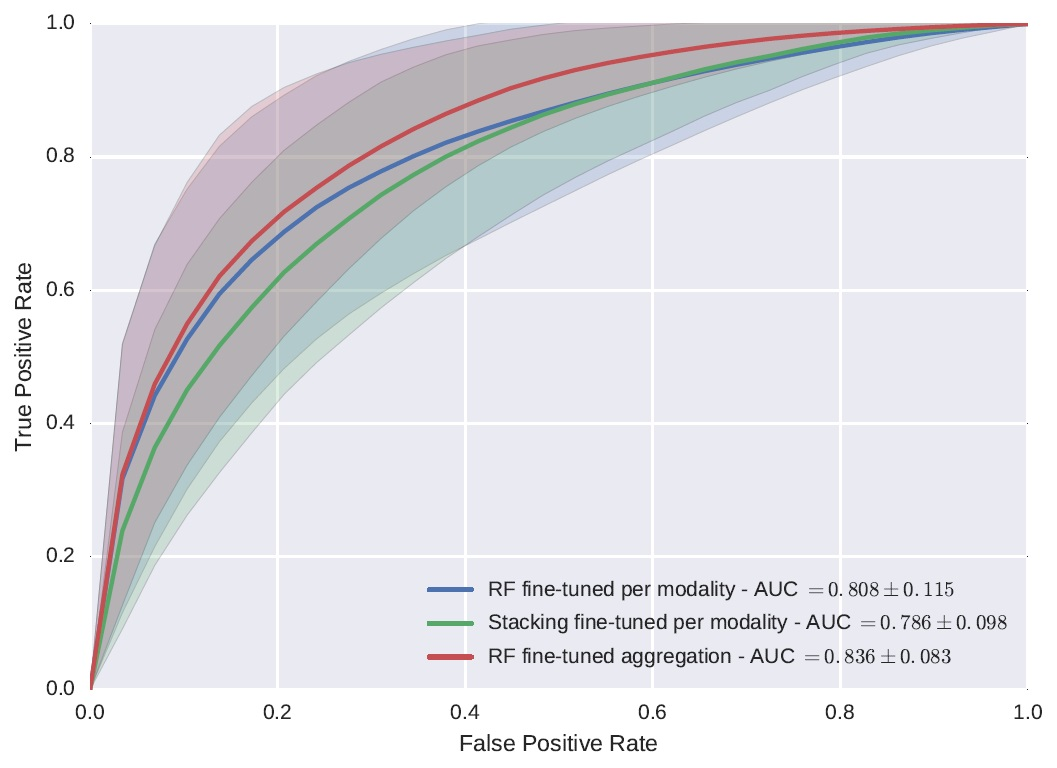
\includegraphics[width=0.9\linewidth]{Figures/test.jpg}
  \caption[Analysis of feature combination approaches after fine tuning.]{Analysis of feature combination approaches after fine tuning through balancing and feature selection/extraction.}
  \label{fig:res-Ex4}
\end{figure}

%\begin{figure}
%  \centering
%  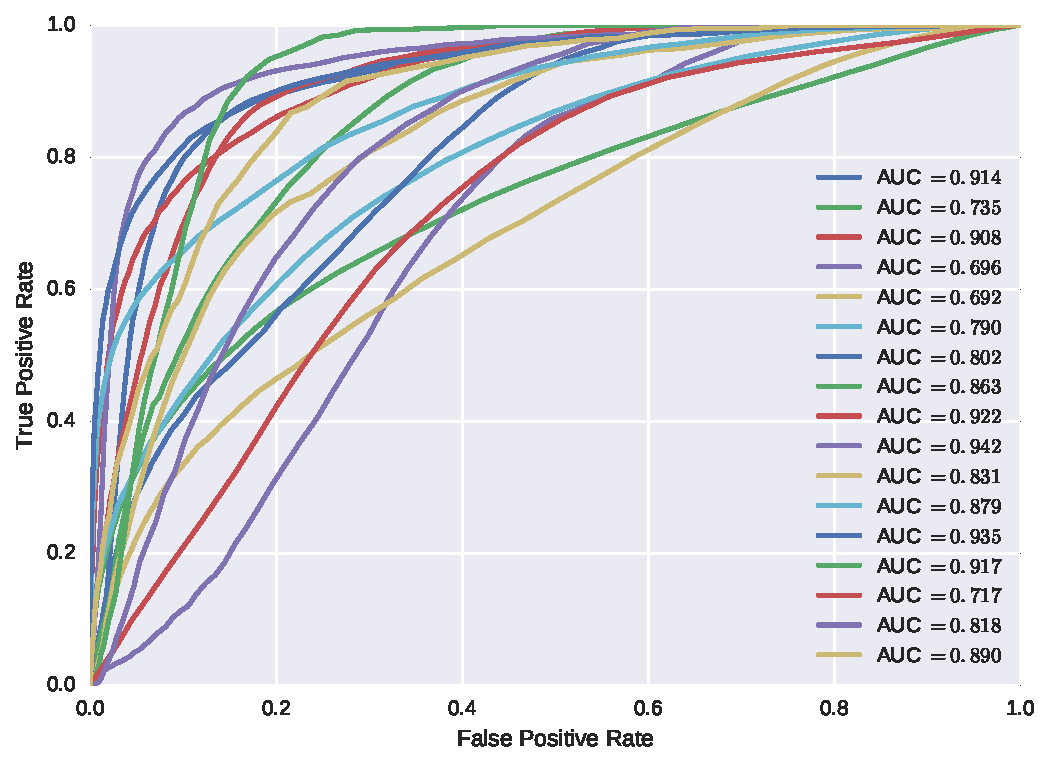
\includegraphics[width=0.7\linewidth]{Figures/plot_all_patients.pdf}
%  \caption{Individual patient \acs*{auc} for the best configuration of the \acs*{mpmri} \acs*{cad}.}
%  \label{fig:indauc}
%\end{figure}
Various experiments were run in order to optimize the balancing and the feature selection strategies  ~\cite{Lemaitre2016thesis}. We found that once all features are concatenated together, \ac{nm3}  ~\cite{mani2003knn} is the method providing the best enhancement of the classification performance with an \ac{auc} of $0.824 \pm 0.076$. Therefore, with this optimal balancing, were here report the final step consisting of three strategies:
(i) the selected features from each modality --- i.e., 331 features --- are concatenated together and used in a \ac{rf} classifier,
(ii) the selected features from each modality --- i.e., 331 features --- are used to train a stacking classifier with a \ac{gb} as meta-classifier, and
(iii) the selected features from the concatenated set of feature --- i.e., 267 features --- are used to train a single \ac{rf} classifier


%\begin{landscape}
\begin{figure}
  %\hspace*{\fill}
  \subfigure[\acs*{auc} = 0.922]{\label{fig:pat634}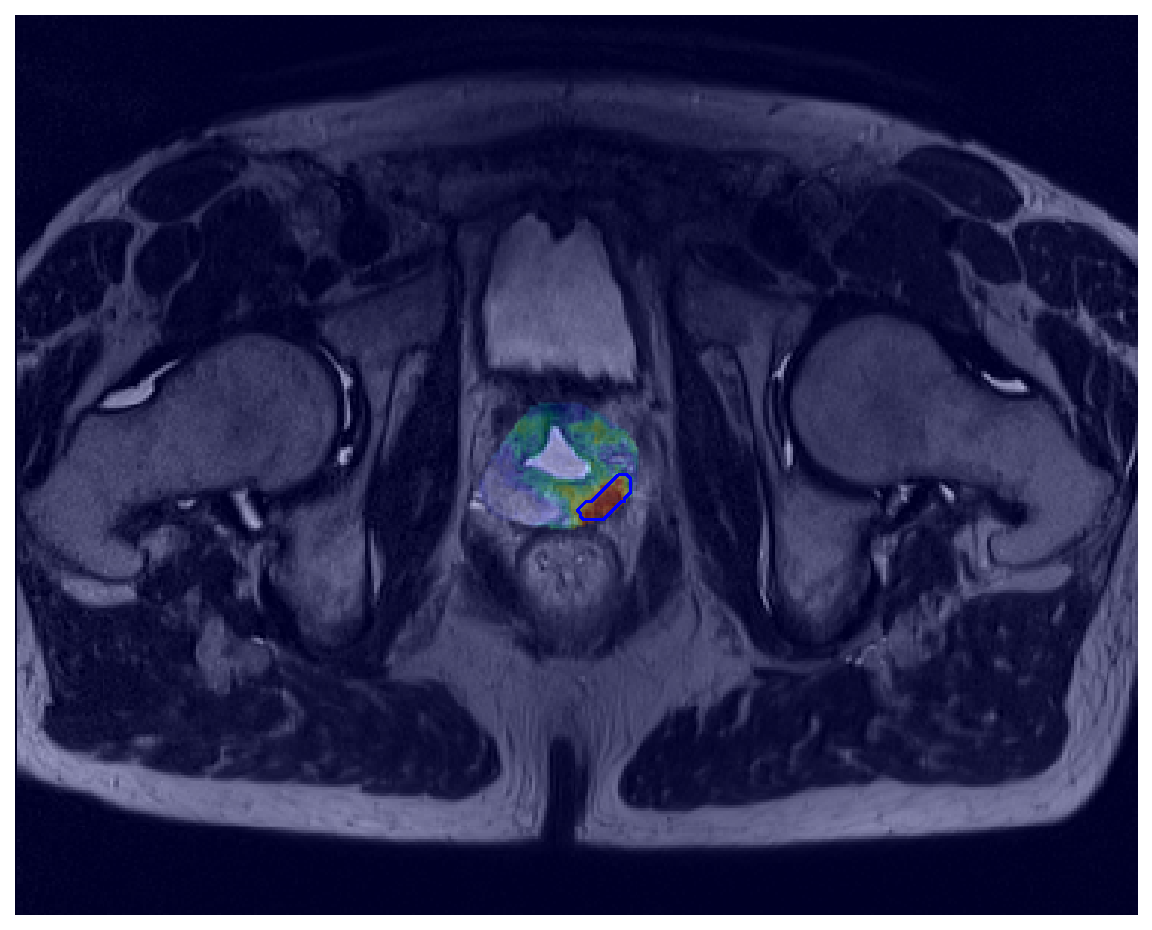
\includegraphics[width=.20\textwidth]{Figures/patient_634.pdf}}
 % \hfill
  \subfigure[\acs*{auc} = 0.942]{\label{fig:pat778}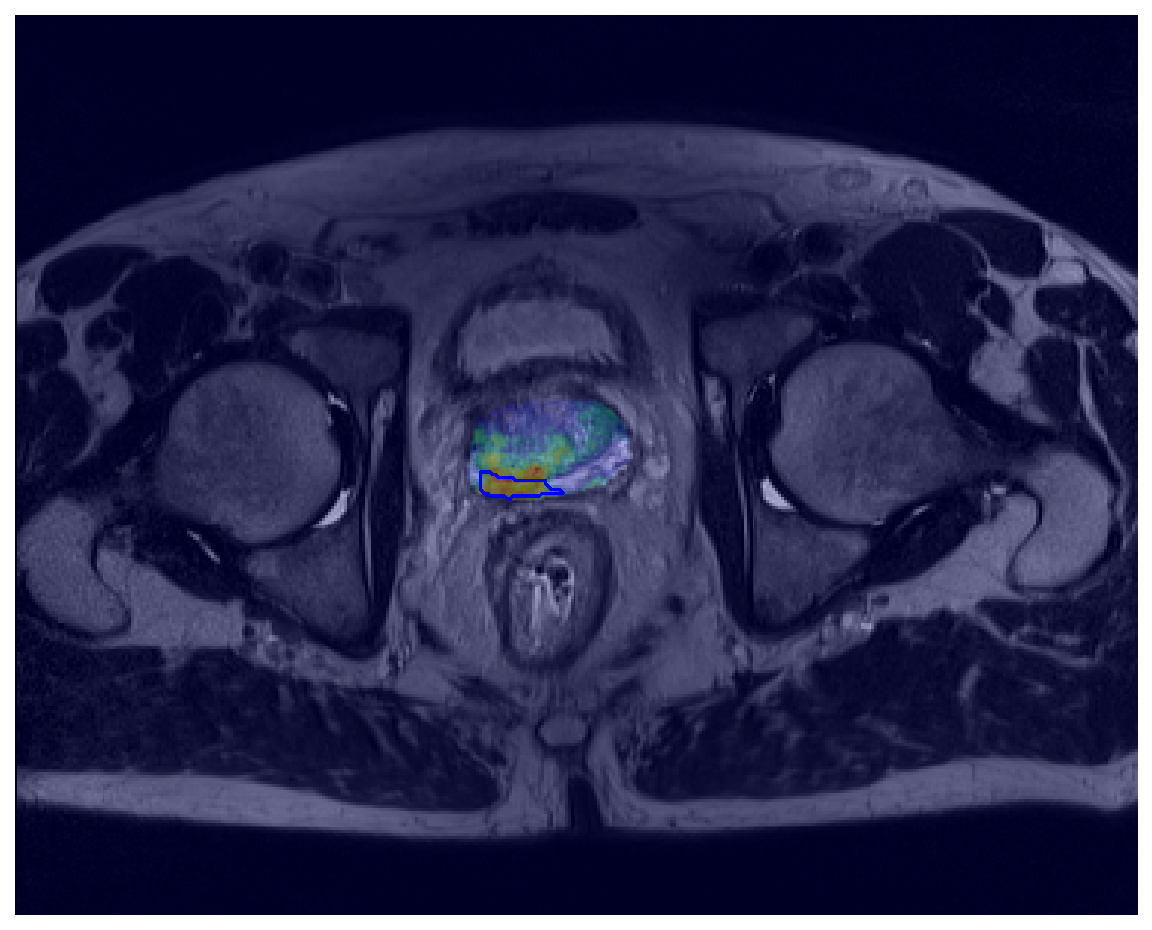
\includegraphics[width=.20\textwidth]{Figures/patient_778.pdf}}
  %\hfill
 % \subfigure[\acs*{auc} = 0.914]{\label{fig:pat1036}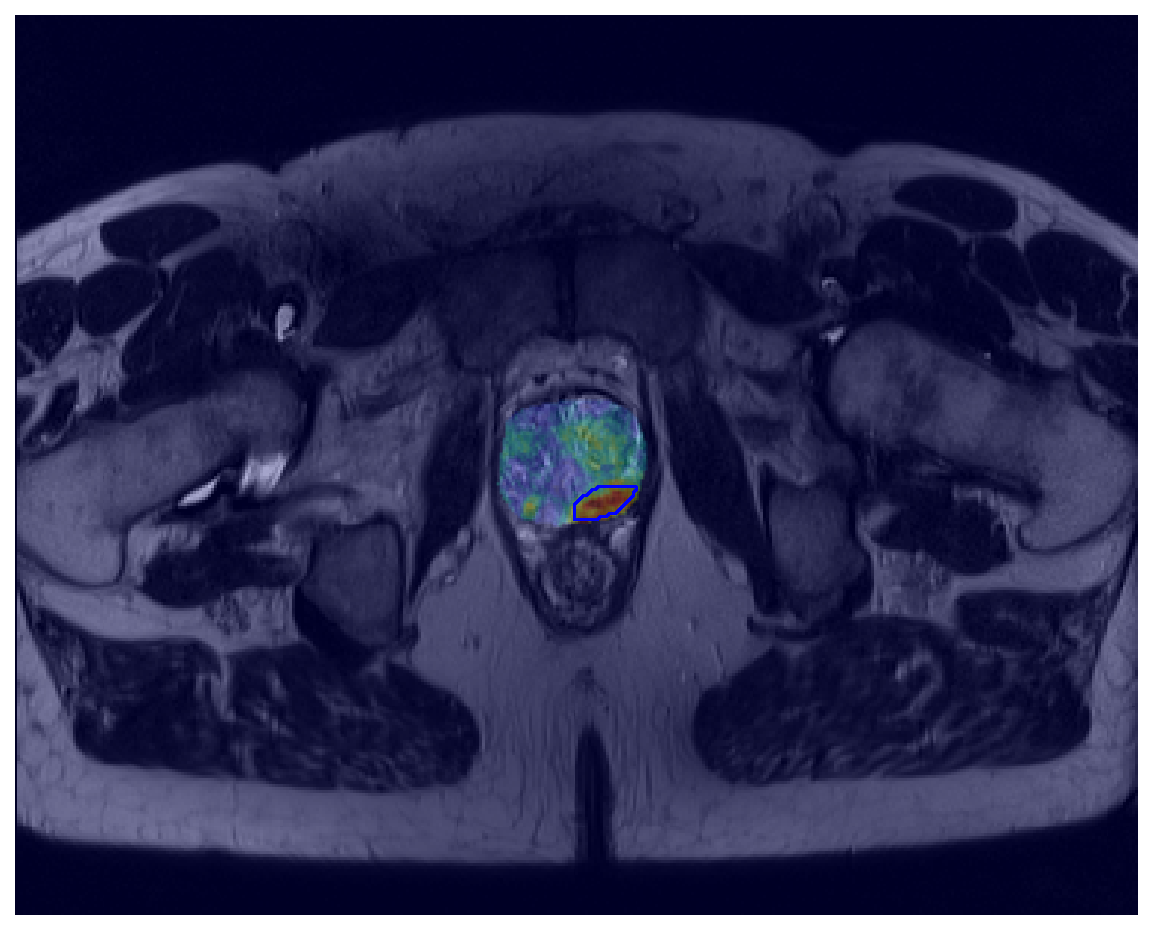
\includegraphics[width=.45\textwidth]{Figures/patient_1036.pdf}}
 % \hspace*{\fill}\\
 % \hspace*{\fill}
%  \subfigure[\acs*{auc} = 0.692]{\label{fig:pat634}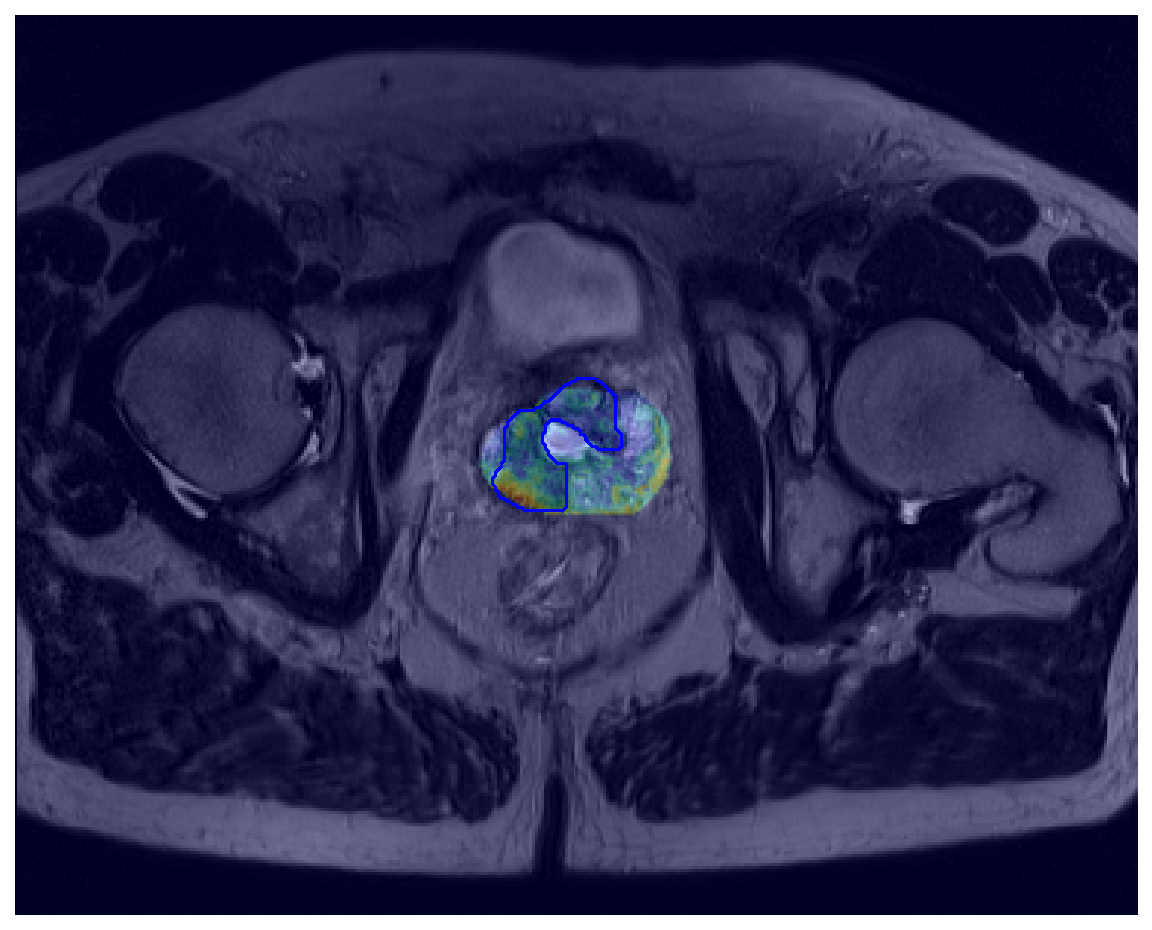
\includegraphics[width=.45\textwidth]{Figures/patient_410.pdf}}
 % \hfill
 % \subfigure[\acs*{auc} = 0.879]{\label{fig:pat778}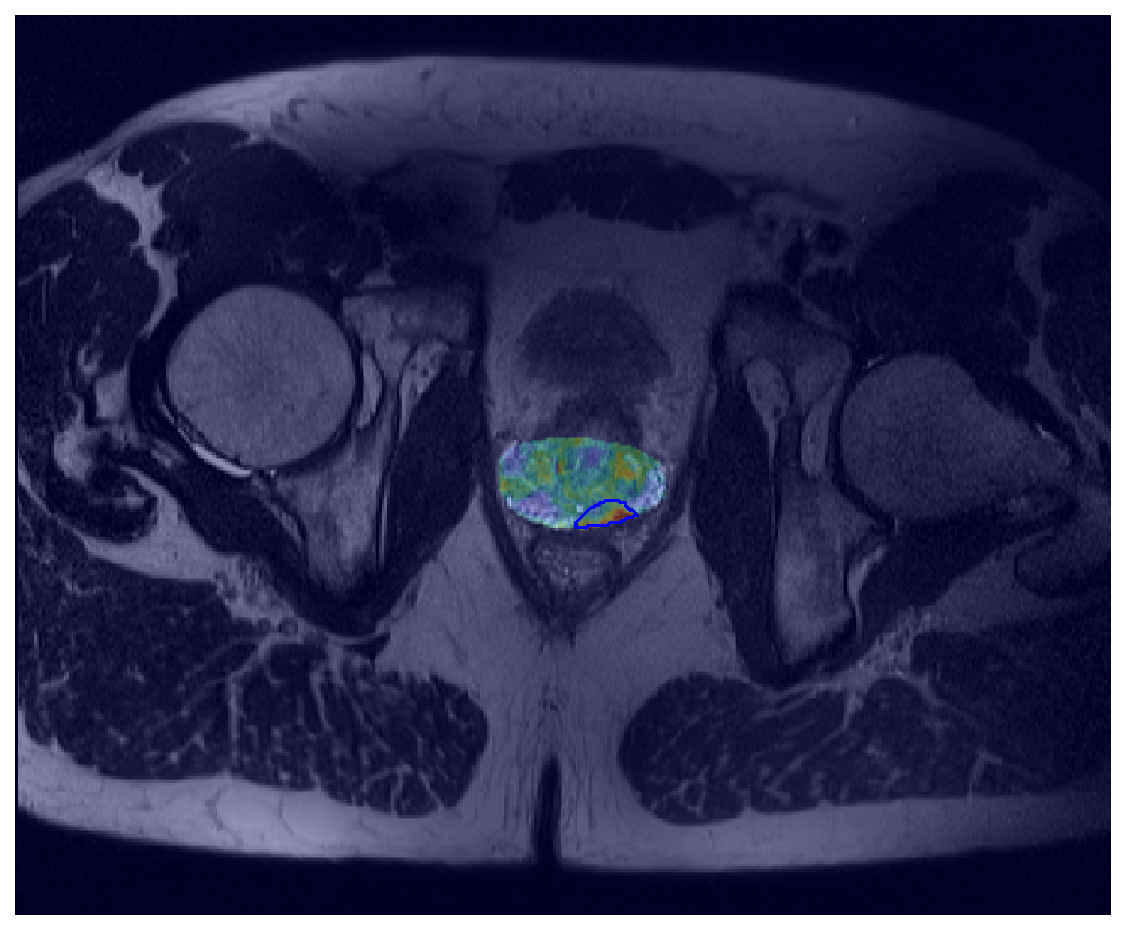
\includegraphics[width=.45\textwidth]{Figures/patient_784.pdf}}
 % \hfill
 % \subfigure[\acs*{auc} = 0.735]{\label{fig:pat1036}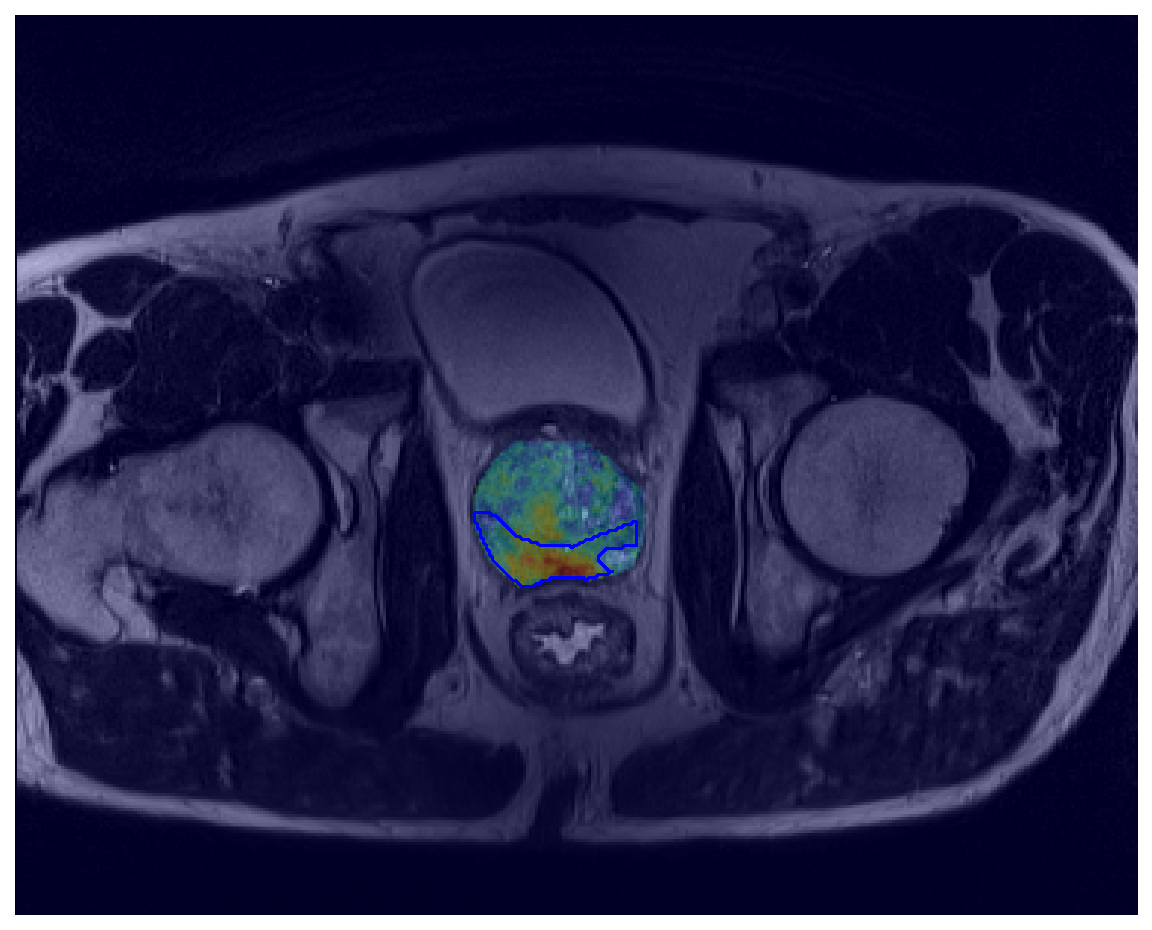
\includegraphics[width=.45\textwidth]{Figures/patient_1041.pdf}}
 % \hspace*{\fill}
  \caption[Illustration the resulting detection of our \acs*{mpmri} \acs*{cad} for \acs*{cap} detection.]{Illustration the resulting detection of our \acs*{mpmri} \acs*{cad} for \acs*{cap} detection. The blue contours corresponds to the \ac{cap} while the jet overlay represents the probability.}
  \label{fig:resultcad}
\end{figure}
%\end{landscape}

The experiment was performed in a \ac{lopo} fashion and a \ac{roc} analysis is carried out.
The comparative results are shown in \acs{fig}\,\ref{fig:res-Ex4}.
In overall, classification using the fine-tuned features improve the classification performance.
The third classification configuration is, however, the one which outperforms others with an \ac{auc} of $0.836 \pm 0.083$.
The improvement in terms of \ac{auc} is of $0.028$ and $0.050$ compared with the 1\textsuperscript{st} and 2\textsuperscript{nd}, respectively.

In clinical setting, the \ac{auc} score is categorized in 3 levels: (i) ``acceptable'' discrimination for an \ac{auc} ranging from $0.7$ to $0.8$, (ii) ``excellent'' discrimination for an \ac{auc} ranging from $0.8$ to $0.9$, and ``outstanding'' discrimination when the \ac{auc} is over $0.9$~\cite{hosmer2004applied}.
Therefore, the combination of all \ac{mri} modalities in conjunction with fine-tuning allow to upgrade our \ac{cad} system from an ``acceptable'' to an ``excellent'' discrimination level.

To illustrate qualitatively the results of our \ac{mpmri} \ac{cad} system, 2 diverse examples are presented in \acs{fig}\,\ref{fig:resultcad} by overlapping the probability map of having a \ac{cap} with the original \ac{t2w}-\ac{mri} slice.
